
%----------------------------------------------------------------
%
%  File    :  komponenten.tex
%
%  Authors :  ???
% 
%  Created :  7 Sept 2019
% 
%  Changed :  7 Sept 2019
% 
%---------------------------------------------------------------


\section{Komponenten}
\label{sec:Komponenten}
	Julian
	\subsection{Use Cases}
	\label{subsec:Use Cases}
	
	Dadurch dass, sich unser 4G LTE Mobilfunknetz über verschiedene Sektoren wie dem Öffentlichen Dienst, der Energieversorgung, dem Transportwesen, wie auch dem Bildungsbereich\cite{Tch18} sowie auch dem Gesundheitswesen erstrecken soll, ergeben sich als Anforderungen vor allem eine hohe Abdeckung, sowie hohe Datenraten, welche für die Benutzer, also die Inselbewohner verfügbar sein sollen. 
	
	Zusätzlich verfügt unsere Insel über ein Seenotrettungssystem präziser gesagt ein maritimes Rettungs-Koordinationszentrum, über welches mit Hilfe von Rettungsschiffen und Rettungsdrohnen in Seenot geratene Inselbewohner lokalisiert werden können \cite{eckermann2018tinylte}. Des weiteren bewegen sich unsere Einwohner auf dem Staatsgebiet der Insel in autonom fahrenden Autos, weshalb auch hierfür entsprechende Anforderungen in Bezug auf die Komponenten für vehikulare Kommunikation eingegangen wird. Da wir eine Infrastruktur von Grund auf erbauen, müssen wir keine Rücksicht auf etwaige bestehende Legacyarchitekturen nehmen, in welche wir neue Komponenten integrieren müssen. 
	\subsection{State of the Art Marktanalyse}
	\label{subsec:Marktanalyse}
	
	Um unsere Inselbewohner zufrieden zustellen, sollten wir insbesondere Peak Data Raten, Zellkapazitäten, den Zellradius, die Radio Access Modi, die Antennen Schemata, sowie das Mobility Speed Handover konkreter in Erwägung ziehen\cite{Dat14}.
	Bei der Recherche zur Thematik haben sich folgende Kriterien als Unterscheidungsmerkmale herauskristallisiert anhand derer letztlich eine Entscheidung getroffen werden soll, ob nun ein Mobilfunknetz selbst errichtet (Make) oder die notwendigen Komponenten (Buy) hinzugekauft werden sollen. Neben dem Spectrum, dem Durchsatz (Throughput), der Latenz (Latency),  der Redundanz (Redundancy), der Interoperabilität beziehungsweise der Kompatibiliät, ist auch die Möglichkeit der Skalierbarkeit, um etwaige Nachbarinseln mitzuversorgen, welche ihrerseits kooperativ Ihre Hilfe in Form eines Internet Cafes angeboten hatten zur Analyse unserer Problematik, sind von signifikanter Bedeutung. Zusätzlich  als weitere nicht zu vernachlässigenden Elemente stellen auch Kritierien wie das des Monitorings respektive des Control Managements, ebenso wie dem möglichen Coverage, als auch die Kapazität  Faktoren dar, welche die finalen Entscheidungsprozesse maßgeblich beeinflussen. Zudem sollte abzuwägen sein, ob ein "Easy to use enerprise Dashboard" vorhanden ist. Des Weiteren ist zu prüfen, ob Lincesing an für sich eine Problematik darstellen könnte. Inwiefern wir auf der Südsee Insel nach internationalem Recht bzw. in welchen gesetzlichen Rahmenbedingungen wir uns bewegen und dementsprechend handeln, sollte ebenfalls noch kurz geklärt werden.
	
	Eine Vielzahl von Anbietern für die Errichtung eines Mobilfunknetzes bestimmen derzeit den globalen LTE Advanced Markt.\ Die dominierenden Unternehmen an diesem sind neben Ambra Solutions, Arris International,
	Athonet, Cisco, Comba, DruidSoftware, Ericsson, Future Technologies, General Dynamics und 
	Huawei. Neben diesen existieren aber auch weitere Anbieter wie beispielsweise Lemko, Luminate Wireless,
	Mavenir,
	NEC,
	Netnumber,
	Nokia,
	Pdvwireless,
	Quortus,
	Redline Communications,
	Samsung,
	Sierra Wireless,
	Star Solutions,
	Ursys,
	Verizon und 
	Zinwave.\cite{Max19}
	
	Abhängig von den Use Cases ergeben sich bei der Analyse und beim Design spezifizierte funktionale wie auch Nicht-funktionale Anforderungen. Haben wir qualifiziertes Fachpersonal geschult auf den LTE Advanced Standard, die sowohl in den Phasen der Anaylse und des Designs als auch in der Implementierung sowie bei Wartung und beim Testen vor Inbetriebnahme gezielt eingesetzt werden können? Haben wir entsprechendes Kapital externer Berater einzufliegen, die schon einmal ähnliche Projekte realisiert haben, um mit Hilfe derer Fehleinschätzungen vergangener Projekte in Bezug auf Planung, Koordination und Aufwandsabschätzungen zu nutzen. Sind generell Fachkräfte mit Know How verfügbar?
	\subsection{HSS, EPC, PCRF}
	\label{subsec:Antennen HSS, EPC, PCRF}
		\subsection{Preise der Komponenten}
	\label{subsec:Preise der Komponenten}
	\subsection{Antennen Konfigurationen}
	\label{subsec:Antennen Konfigurationen}
Bevor man die Komponenten, welche von unterschiedlichen Marktteilnehmern angeboten vergleicht, muss man sich ein Bild über die Empfangsbedingungen in unserem Inselstaat machen. Abhängig von physikalischen Einflussfaktoren in Form von Waldgebieten, Gebäude komplexen, topologische Strukturen wie Gebirge können signifikant die Signalübertragung bestimmen. Denn schließlich sind Absorption, Beugung oder auch Reflexion mit die Hauptgründe für Störungen bei der Ausbreitung elektromagnetischer Wellen. Um nun einen optimalen Empfang zu gewähren kann eine Kombination aus Antennentypen angedacht werden, da jede einzelne Bauart ihre Vor- und Nachteile aufweist. So ist zu unterscheiden zwischen Mono-und Breitband Antennen. Monoantennen sind hierbei der Klasse der Richtantennen und Breitbandantennen der Klasse der Rundstrahler zuzuordnen. \cite{Sch19}
\begin{figure}[H]
	\centering
	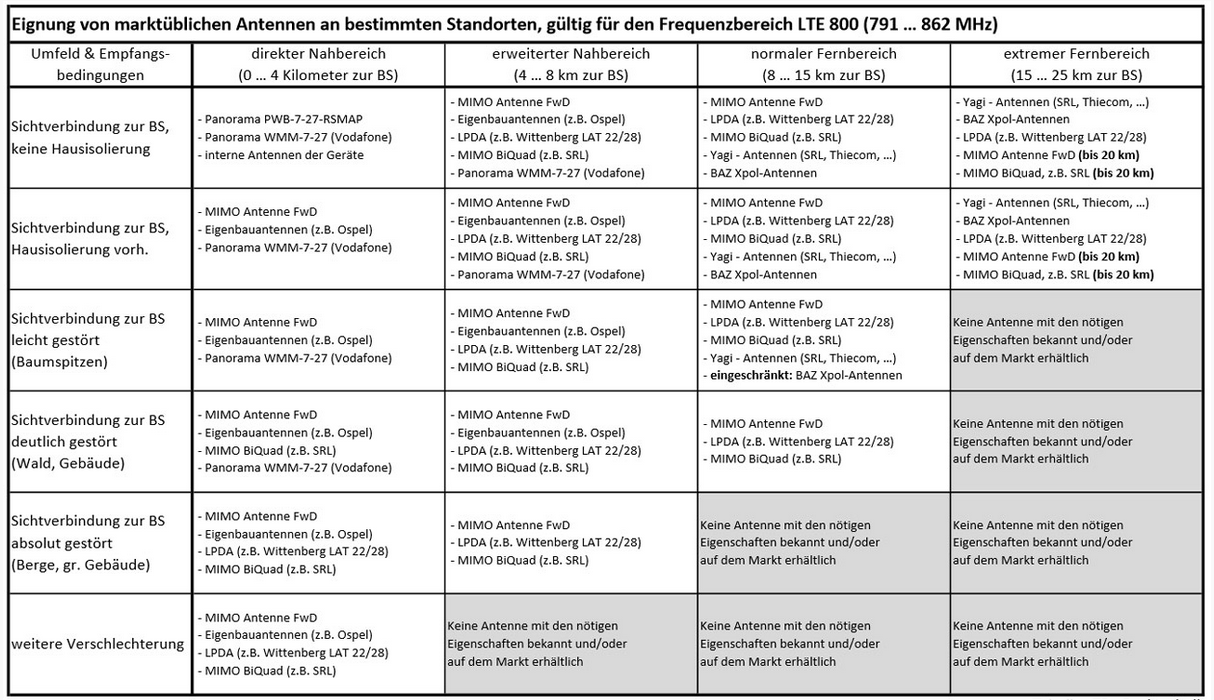
\includegraphics[width=1\linewidth]{images/tabellemcnantennen}
	\caption{Antennenüberblick  \protect\cite{Sch19}}
	\label{fig:tabellemcnantennen}
\end{figure}
 %\flushbottom 
%\nextpage
\raggedbottom 
